\section{Experiment 3}\label{sec:experiment-3}
This experiment is targetted towards \gls{pca} and \gls{kpca}. The goal is to compare the performance of \gls{pca} and \gls{kpca}, because these methods are similar, with the exception that \gls{kpca} implements a kernel. Beause of the similarity of the methods, comparison will be more focused on the impact the different kernels can have on the model, namely what numbers does the machine learning model confuse given the different kernels.


As explained in the Chapter Theory, KPCA can have kernels, which will project the data into a higher dimensional feature space, where a hyperplane can be constructed, and perform PCA on it. KPCA does not require the transformation of the inputs into the feature space with the kernel function, but can use the kernels so as to get the dot product of the pair-wise input points~\cite{kpca-book}.


The kernels are a measure of similarity between the points~\cite{scikit-learn}, which means that points that are close to each other have higher similarity score, which is computed with the kernel function. The kernels chosen for the experiment are the \gls{rbf} and sigmoid kernels. The sigmoid kernel \textcquote{scikit-learn}{computes the sigmoid kernel between two vectors}, which outputs a value between -1 and 1 for the two given input vectors. The \gls{rbf} kernel \textcquote{scikit-learn}{computes the radial basis function kernel between two vectors}, which outputs a value between 0 and 1.


\subsection{Rules}
This experiment will not use gridsearch. The input of the data samples will be 15000 for both of the methods, because of hardware limitations. The amount of components used for the methods will be the ones that were used in experiment one, namely 49 components. The evaluation will be based on the confusion matrices. The kernels used will be \gls{rbf} and sigmoid. The experiment will be run on the hardware described in Table~\ref{tab:pc2-specs}.

\subsection{Results}
Figure \ref{fig:confusion-matrix-pca-svm} shows the results for \gls{pca}.
Figure~\ref{fig:confusion-matrix-kernel-pca-svm-sigmoid} shows the results for \gls{kpca} with sigmoid kernel.
Figure~\ref{fig:confusion-matrix-kernel-pca-svm-rbf} shows the results for \gls{kpca} with rbf kernel.


\begin{figure}[htb!]
    \centering
    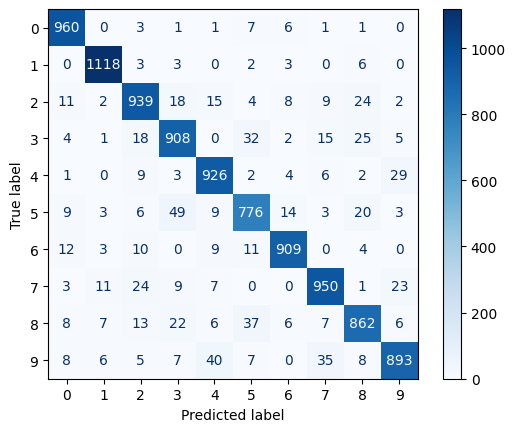
\includegraphics[width=0.5\textwidth]{../src/results/experiment_three/confusion_matrix_pca_svm.png}
    \caption{Confusion matrix for PCA}
    \label{fig:confusion-matrix-pca-svm}
\end{figure}



\begin{figure}
    \centering
    \subfloat[\centering Confusion matrix for kPCA Sigmoid]{\label{fig:confusion-matrix-kernel-pca-svm-sigmoid}{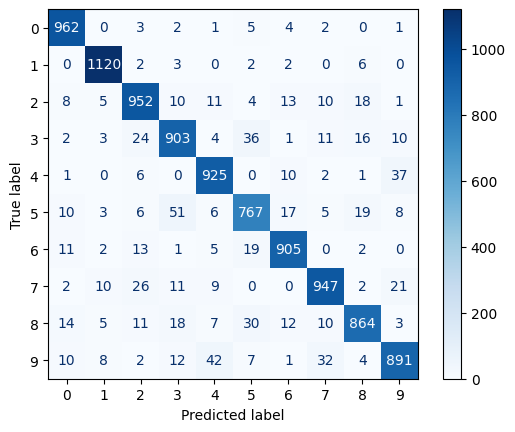
\includegraphics[width=0.45\textwidth]{../src/results/experiment_three/confusion_matrix_kernel_pca_svm_sigmoid.png} }}
    \qquad
    \subfloat[\centering Confusion matrix for kPCA RBF]{\label{fig:confusion-matrix-kernel-pca-svm-rbf}{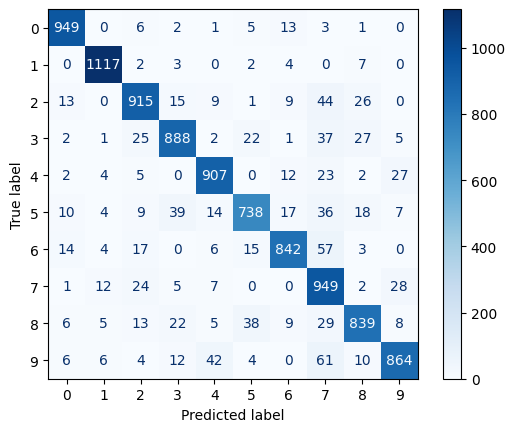
\includegraphics[width=0.45\textwidth]{../src/results/experiment_three/kernel_pca_rbf_kernel_49.png} }}%
    \caption{both kPCA kernels confusion matrices}
    \label{fig:kpca-kernels}
\end{figure}


\subsection{Results}
From the results presented so far about the differences between the kernels it can be seen that all the methods often confuse the number 2 with 8; 3 with 2,5,8 and to a certain degree(PCA and much worse with \gls{kpca-r}), 7. The methods also confuse the number 4 with 9; 5 with 3,6, and 8 (\gls{kpca-r} also does it with 7). The number 6 gets confused with the number 0,2,5 (\gls{kpca-r} also does it with 7).
The number 7 gets confused with the number 2,3 and 9. \gls{kpca-r} is the only one that did not confuse the number 3 as much as the other methods.

At number 8, the methods have confused 0 (except for \gls{kpca-r}),2,3 and 5. \gls{kpca-r} confused it again with the number 7, but it is the only one that managed to map the number 0 less than the other methods. Lastly the number 9 got confused with the numbers the most with the numbers 4 and 7. It can be further noted that \gls{kpca-r} is the worst at confusing various numbers with the number 7.

\subsection{Discussion of results}
From the overview provided regarding the difference in numbers, a percentage would be more preferable, more specifically, a percentage of the errors made in the numbers 0-9. The error percentage can be calculated the number of current correct predictions divided by the total number of numbers from the given class. Table \ref{tab:error-percentage-pca-kpca-s-kpca-r} shows the difference in percentages of errors made by the methods for each number.

\begin{table}[htb!]
    \centering
    \begin{tabular}{lrrrr}
        \toprule
          & pca    & kpca-s & kpca-r \\
        \midrule
        0 & 2.959  & 1.836  & 3.163  \\
        1 & 1.585  & 1.321  & 1.585  \\
        2 & 8.817  & 7.751  & 11.337 \\
        3 & 10.594 & 10.594 & 12.079 \\
        4 & 5.702  & 5.804  & 7.637  \\
        5 & 12.556 & 14.013 & 17.264 \\
        6 & 6.054  & 5.532  & 12.108 \\
        7 & 7.101  & 7.879  & 7.684  \\
        8 & 13.552 & 11.293 & 13.860 \\
        9 & 11.992 & 11.694 & 14.370 \\
        \bottomrule
    \end{tabular}
    \caption{Error percentage for each number for the methods}
    \label{tab:error-percentage-pca-kpca-s-kpca-r}
\end{table}


With the help of the table, it can be seen that \gls{kpca-r} has an overall worse performance than \gls{kpca-s}. The differences between those two methods in relation to the error percentage presented in \gls{pca} is presented in Table~\ref{tab:error-percentage-difference-pca-kpca-s-kpca-r}.

\begin{table}[htb!]
    \centering
    \begin{tabular}{lrrrr}
        \toprule
           & kpca-s & kpca-r    \\
        \midrule
        0  & -1.123  & +0.204   \\
        1  & -0.264  & 0        \\
        2  & -1.066  & +2.52    \\
        3  &  0      & +1.485   \\
        4  & +0.102  & +1.935   \\
        5  & +1.457  & +4.708   \\
        6  & -0.522  & +6.054   \\
        7  & +0.778  & +0.583   \\
        8  & -2.259  &  +0.308  \\
        9  & -0.298  & +2.378   \\
        \bottomrule
    \end{tabular}
    \caption{Difference between the error percentage for the kernels compared to pca. The difference is calculated by subtracting the error percentage of the kernel from the error percentage of pca.}
    \label{tab:error-percentage-difference-pca-kpca-s-kpca-r}
\end{table}

Based on the tables~\ref{tab:error-percentage-pca-kpca-s-kpca-r} and \ref{tab:error-percentage-difference-pca-kpca-s-kpca-r} it seems as if \gls{kpca-r} predicts too many times the number 7 for various numbers, which is a reason for why \gls{kpca-s} is better than \gls{kpca-r}.


